% =====================================================================
% BMED365 (Spring 2027) — Lab 4: Differentiable Neurosymbolic AI Report
% Printable Companion Notebook Export: 03_multiseed_ablation_and_calibration.ipynb
% Compile with: pdflatex 03_multiseed_ablation_and_calibration_ipynb.tex (run twice)
% =====================================================================
\documentclass[10pt,a4paper]{article}

\usepackage[utf8]{inputenc}
\usepackage[T1]{fontenc}
\usepackage[english]{babel}
\usepackage{lmodern}
\usepackage{microtype}
\usepackage{graphicx}
\usepackage{booktabs}
\usepackage{xltabular}
\usepackage{tabularx}
\usepackage{array}
\usepackage[table]{xcolor}
\usepackage{amsmath,amssymb,mathtools}
\usepackage{enumitem}
\usepackage[margin=1.7cm,top=1.75cm,bottom=1.85cm,headheight=14pt]{geometry}
\usepackage{fancyhdr}
\usepackage{lastpage}
\usepackage{titlesec}
\usepackage[most]{tcolorbox}
\usepackage{listings}
\usepackage{float}
\usepackage{caption}
\usepackage[hyphens]{url}
\usepackage[
    colorlinks=true,
    linkcolor=uibblue,
    citecolor=uibblue,
    urlcolor=uibred,
    bookmarksnumbered=true,
    bookmarksopen=true,
    pdftitle={03_multiseed_ablation_and_calibration.ipynb -- Multi-Seed Controlled 6-Model Ablation and Calibration (BMED365 Spring 2027)},
    pdfauthor={Arvid Lundervold (University of Bergen & MMIV) -- BMED365 Spring 2027},
    pdfsubject={BMED365 Spring 2027 -- Differentiable Neurosymbolic AI Companion Notebook}
]{hyperref}
\def\UrlBreaks{\do\/\do-\do_\do.}
% Allow clean line breaks after underscores in long filenames & Python identifiers
\let\origunderscore\_
\renewcommand{\_}{\origunderscore\allowbreak}

% =====================================================================
% COLORS (UiB / MMIV / BMED365 House Style)
% =====================================================================
\definecolor{uibblue}{RGB}{0, 61, 115}
\definecolor{uibred}{RGB}{175, 28, 44}
\definecolor{kiwigreen}{RGB}{27, 138, 90}
\definecolor{amberwarn}{RGB}{165, 95, 0}
\definecolor{amberbg}{RGB}{255, 250, 240}
\definecolor{lightgray}{RGB}{246, 248, 250}
\definecolor{rowalt}{RGB}{243, 247, 252}
\definecolor{codebg}{RGB}{245, 248, 252}
\definecolor{codehdr}{RGB}{224, 234, 246}
\definecolor{outbg}{RGB}{250, 250, 250}
\definecolor{outhdr}{RGB}{236, 238, 240}
\definecolor{codekw}{RGB}{0, 75, 145}
\definecolor{codestr}{RGB}{155, 35, 45}
\definecolor{codecmt}{RGB}{90, 105, 118}

% =====================================================================
% TYPOGRAPHY, HEADERS & CALLOUT BOXES
% =====================================================================
\setlength{\parindent}{0pt}
\setlength{\parskip}{0.42em}
\setlength{\emergencystretch}{1.8em}
\setlist[itemize]{topsep=2pt,itemsep=2pt,leftmargin=1.45em}
\setlist[enumerate]{topsep=2pt,itemsep=2pt,leftmargin=1.65em}

\newcolumntype{L}[1]{>{\raggedright\arraybackslash}p{#1}}
\newcolumntype{C}[1]{>{\centering\arraybackslash}p{#1}}
\newcolumntype{R}[1]{>{\raggedleft\arraybackslash}p{#1}}
\newcolumntype{Y}{>{\raggedright\arraybackslash}X}

\titleformat{\section}{\large\bfseries\color{uibblue}}{\thesection}{0.65em}{}[\vspace{1pt}\color{uibblue!40}\titlerule]
\titleformat{\subsection}{\normalsize\bfseries\color{uibblue!88!black}}{\thesubsection}{0.55em}{}
\titleformat{\subsubsection}{\small\bfseries\color{uibblue!75!black}}{\thesubsubsection}{0.5em}{}
\titlespacing*{\section}{0pt}{1.05em}{0.4em}
\titlespacing*{\subsection}{0pt}{0.75em}{0.25em}
\titlespacing*{\subsubsection}{0pt}{0.55em}{0.2em}

\pagestyle{fancy}
\fancyhf{}
\fancyhead[L]{\footnotesize\textcolor{gray}{BMED365 (Spring 2027) $\cdot$ Neurosymbolic 7\,T MRI Package}}
\fancyhead[R]{\footnotesize\textcolor{gray}{\texttt{03\_multiseed\_ablation\_and\_calibration.ipynb}}}
\fancyfoot[L]{\footnotesize\textcolor{gray}{University of Bergen \& MMIV $\cdot$ \href{https://github.com/arvidl/BMED365-2027}{\textcolor{gray}{github.com/arvidl/BMED365-2027}}}}
\fancyfoot[R]{\footnotesize\textcolor{gray}{Page \thepage{} of \pageref{LastPage}}}
\renewcommand{\headrulewidth}{0.4pt}
\renewcommand{\footrulewidth}{0.2pt}

\fancypagestyle{firstpage}{
    \fancyhf{}
    \fancyfoot[L]{\footnotesize\textcolor{gray}{University of Bergen \& MMIV $\cdot$ \href{https://github.com/arvidl/BMED365-2027}{\textcolor{gray}{github.com/arvidl/BMED365-2027}}}}
    \fancyfoot[R]{\footnotesize\textcolor{gray}{Page \thepage{} of \pageref{LastPage}}}
    \renewcommand{\headrulewidth}{0pt}
    \renewcommand{\footrulewidth}{0.2pt}
}

% --- Notebook Cell & Pedagogical Boxes ---
\newtcolorbox{seqbox}[1][]{
    enhanced, breakable,
    colback=lightgray, colframe=uibblue,
    colbacktitle=uibblue, coltitle=white,
    fonttitle=\bfseries\small, title={#1},
    boxrule=0.6pt, arc=2.5pt, left=7pt, right=7pt, top=5pt, bottom=5pt
}

\newtcolorbox{codebox}[1][]{
    enhanced, breakable,
    colback=codebg, colframe=uibblue!35,
    colbacktitle=codehdr, coltitle=uibblue!90!black,
    fonttitle=\ttfamily\scriptsize\bfseries, title={#1},
    boxrule=0.55pt, arc=2.2pt, left=6pt, right=6pt, top=3pt, bottom=3pt,
    toptitle=2.5pt, bottomtitle=2.5pt
}

\newtcolorbox{outbox}[1][]{
    enhanced, breakable,
    colback=outbg, colframe=gray!45,
    colbacktitle=outhdr, coltitle=black!75,
    fonttitle=\ttfamily\scriptsize\bfseries, title={#1},
    boxrule=0.5pt, arc=2.2pt, left=6pt, right=6pt, top=3pt, bottom=3pt,
    toptitle=2pt, bottomtitle=2pt
}

\newtcolorbox{clinbox}[1][]{
    enhanced, breakable,
    colback=amberbg, colframe=amberwarn,
    colbacktitle=amberwarn, coltitle=white,
    fonttitle=\bfseries\small, title={#1},
    boxrule=0.6pt, arc=2.5pt, left=7pt, right=7pt, top=5pt, bottom=5pt
}

\newtcolorbox{guidehdr}[1][]{
    enhanced,
    colback=kiwigreen!6, colframe=kiwigreen!75!black,
    borderline west={2.5pt}{0pt}{kiwigreen!85!black},
    boxrule=0.45pt, arc=2pt, left=7pt, right=7pt, top=3.5pt, bottom=3.5pt,
    before skip=0.7em, after skip=0.35em
}

% --- Listings Styles (UTF-8 literate support for pdflatex) ---
\lstdefinestyle{pybmed}{
    language=Python,
    basicstyle=\ttfamily\scriptsize,
    keywordstyle=\bfseries\color{codekw},
    stringstyle=\color{codestr},
    commentstyle=\itshape\color{codecmt},
    showstringspaces=false,
    breaklines=true,
    breakatwhitespace=false,
    breakindent=12pt,
    columns=fullflexible,
    keepspaces=true,
    upquote=true,
    aboveskip=2pt,
    belowskip=2pt,
    xleftmargin=0pt,
    xrightmargin=0pt,
    literate={±}{{$\pm$}}1
             {³}{{\textsuperscript{3}}}1
             {×}{{$\times$}}1
             {é}{{\'e}}1
             {ö}{{\"o}}1
             {Ł}{{\L{}}}1
             {Δ}{{$\Delta$}}1
             {α}{{$\alpha$}}1
             {–}{{--}}1
             {—}{{---}}1
             {≥}{{$\ge$}}1
             {≤}{{$\le$}}1
             {⊂}{{$\subset$}}1
             {∈}{{$\in$}}1
             {→}{{$\to$}}1
             {…}{{\ldots}}1
}

\lstdefinestyle{bashbmed}{
    language=bash,
    basicstyle=\ttfamily\scriptsize,
    keywordstyle=\bfseries\color{codekw},
    stringstyle=\color{codestr},
    commentstyle=\itshape\color{codecmt},
    showstringspaces=false,
    breaklines=true,
    breakatwhitespace=false,
    breakindent=12pt,
    columns=fullflexible,
    keepspaces=true,
    upquote=true,
    aboveskip=2pt,
    belowskip=2pt,
    xleftmargin=0pt,
    xrightmargin=0pt
}

\lstdefinestyle{outbmed}{
    basicstyle=\ttfamily\scriptsize\color{black!85},
    showstringspaces=false,
    breaklines=true,
    breakatwhitespace=false,
    columns=fullflexible,
    keepspaces=true,
    upquote=true,
    aboveskip=1pt,
    belowskip=1pt,
    xleftmargin=0pt,
    xrightmargin=0pt
}

\lstdefinestyle{outbmedwide}{
    basicstyle=\ttfamily\fontsize{6.3pt}{7.6pt}\selectfont\color{black!85},
    showstringspaces=false,
    breaklines=true,
    breakatwhitespace=false,
    columns=fullflexible,
    keepspaces=true,
    upquote=true,
    aboveskip=1pt,
    belowskip=1pt,
    xleftmargin=0pt,
    xrightmargin=0pt
}

\newcommand{\ghblob}{https://github.com/arvidl/BMED365-2027/blob/main}
\newcommand{\colabbase}{https://colab.research.google.com/github/arvidl/BMED365-2027/blob/main}
\newcommand{\repodir}{Lab4-Comp-Imag/Kiwi-challenge/docs/neurosymbolic-report}
\newcommand{\colabbtn}[1]{%
  \href{#1}{\tcbox[on line, arc=2.5pt, boxsep=0pt, left=6pt, right=6pt, top=2.5pt, bottom=2.5pt,
    colback=amberwarn!85!yellow, colframe=white!70!amberwarn, boxrule=0.5pt]{%
    \sffamily\bfseries\scriptsize\color{white}Open in Google Colab}}%
}

% =====================================================================
\begin{document}
\thispagestyle{firstpage}

% --- TITLE BANNER ---
\begin{tcolorbox}[
    enhanced, colback=uibblue, colframe=uibblue,
    arc=3.5pt, left=12pt, right=12pt, top=9pt, bottom=9pt
]
{\Large\bfseries\color{white} Companion Notebook 03 --- Multi-Seed Controlled 6-Model Ablation \& Calibration\\[2pt]
{\large 3-Seed Unmasked 3D Panoptic Quality Benchmark, Operating-Point Calibration \& Whole-Organ OOD Safety}}\\[4pt]
{\normalsize\color{white!90} BMED365 --- Computational Imaging, Modeling and AI in Biomedicine (Spring 2027)}\\[3pt]
{\footnotesize\color{white!84}
Arvid Lundervold (University of Bergen \& MMIV) $\;\cdot\;$ Reproduces Report Sec.\ 3.3, Figs.\ 6--7 \& Tables~5--6 $\;\cdot\;$ Measured runtime: \texttt{555.1 s} (MPS)
}\\[6pt]
\colabbtn{\colabbase/\repodir/notebooks/03_multiseed_ablation_and_calibration.ipynb}\hspace{8pt}
{\footnotesize\href{\ghblob/\repodir/notebooks/03_multiseed_ablation_and_calibration.ipynb}{\textcolor{white}{\underline{\texttt{03\_multiseed\_ablation\_and\_calibration.ipynb} on GitHub}}}}\hspace{10pt}
{\footnotesize\href{\ghblob/\repodir/neurosymbolic-kiwi-report.pdf}{\textcolor{white}{\underline{Technical Report PDF}}}}
\end{tcolorbox}

\begin{seqbox}[Neurosymbolic 7\,T MRI Technical Report --- Companion Package (\texttt{docs/neurosymbolic-report})]
{\footnotesize Companion to \href{\ghblob/\repodir/neurosymbolic-kiwi-report.pdf}{\textbf{\texttt{neurosymbolic-kiwi-report.pdf}}} and shared library \href{\ghblob/\repodir/notebooks/kiwi_ns_lib.py}{\texttt{kiwi\_ns\_lib.py}} (\href{\ghblob/\repodir/notebooks/kiwi_ns_lib_py.pdf}{\textit{annotated PDF}}):}
\begin{enumerate}[start=1, itemsep=1.2pt, topsep=2pt, font=\footnotesize]
    \item \href{\ghblob/\repodir/notebooks/01_data_geometry_and_prior_audit.ipynb}{\texttt{01\_data\_geometry\_and\_prior\_audit.ipynb}} --- 7\,T MRI geometry, empirical audit of Priors 1--3, tri-planar Micro-GT superimposition \& manual GT editing guide (Figs.\ 1--3, Table~3; 27.4\,s MPS).
    \item \href{\ghblob/\repodir/notebooks/02_instancenorm_trap_and_ltn_math.ipynb}{\texttt{02\_instancenorm\_trap\_and\_ltn\_math.ipynb}} --- Experimental proof of \texttt{InstanceNorm3d} coordinate erasure, Bayes Log-Odds \texttt{Organ-GPS}, fuzzy $T$-norms \& LTN $p$-mean autograd sweep (Figs.\ 4--5, Table~4; 7.2\,s MPS).
    \item \textbf{\texttt{03\_multiseed\_ablation\_and\_calibration.ipynb} (this notebook)} --- 3-seed $\times$ 6-model controlled ablation, operating-point calibration shift \& unmasked whole-organ OOD safety (Figs.\ 6--7, Tables~5--6; 555.1\,s MPS).
    \item \href{\ghblob/\repodir/notebooks/04_mechanistic_interpretability_and_biomarkers.ipynb}{\texttt{04\_mechanistic\_interpretability\_and\_biomarkers.ipynb}} --- Causal neural--symbolic division of labor ($z_{\text{GPS}}$), Mat\'ern hard-core split sweep, error anatomy \& 128-slice NIfTI biomarkers (Figs.\ 8--9, Tables~7--8; 99.3\,s MPS).
    \item \href{\ghblob/\repodir/notebooks/05_axiom_stress_tests_and_clinical_translation.ipynb}{\texttt{05\_axiom\_stress\_tests\_and\_clinical\_translation.ipynb}} --- Pathological mass-effect center-shift ($\Delta r \in [0, 8]$\,mm) \& radial-scale ($\alpha \in [0.80, 1.25]$) stress tests vs.\ rigid post-hoc masks (Fig.\ 10, Table~9; 55.4\,s MPS).
\end{enumerate}
\end{seqbox}

\subsection*{Purpose}
To achieve Master's-thesis statistical rigor, we evaluate \textbf{six controlled architectures /\allowbreak{} logic regimes} across \textbf{3 independent random seeds (\texttt{SEEDS = [2027, 2028, 2029]})} with \textbf{ZERO post-hoc test masks}:
\begin{itemize}
\item \textbf{A.} Supervised 3D Multi-Task U-Net Baseline (\texttt{thr = 0.50})
\item \textbf{B.} Naive \texttt{CoordConv3D} (\texttt{InstanceNorm3d}) + LTN (\texttt{p = 3})
\item \textbf{C.} Additive Bayes \texttt{Organ-GPS} + Arithmetic-Mean Logic (\texttt{p = 1})
\item \textbf{D.} Additive Bayes \texttt{Organ-GPS} + Quadratic Logic (\texttt{p = 2})
\item \textbf{E.} Additive Bayes \texttt{Organ-GPS} + LTN (\texttt{p = 3}, evaluated both uncalibrated \texttt{0.42} and train-calibrated + \texttt{Lab 5} hard-core split)
\item \textbf{F.} Coupled Concat \texttt{Organ-GPS} + LTN (\texttt{p = 3}, train-calibrated + \texttt{Lab 5} hard-core split --- NB 06 fusion style)
\end{itemize}

\textit{(Tip: Runs all 3 seeds in \texttt{\textasciitilde{}4--5 min} on Apple Silicon \texttt{mps} or Colab \texttt{T4} GPU; change \texttt{SEEDS = [2027]} for a fast \texttt{\textasciitilde{}90 s} classroom run.)}

\section*{0. Environment Setup: Portable Execution, Shared Training Harness \& Accelerator Selection}
\addcontentsline{toc}{section}{\texorpdfstring{0. Environment Setup: Portable Execution, Shared Training Harness \& Accelerator Selection}{0. Environment Setup: Portable Execution, Shared Training Harness and Accelerator Selection}}

\begin{guidehdr}
{\small\bfseries\color{kiwigreen!75!black}Conceptual \& Practical Motivation}
\end{guidehdr}
This notebook trains \textbf{3 self-supervised 3D warm-start backbones} and \textbf{18 full 3D segmentation models} (6 controlled variants $\times$ 3 independent random seeds) and evaluates every model unmasked over all $256 \times 256 \times 128$ voxels. The setup cell prepares a reproducible environment across local and Colab sessions:

\begin{itemize}
\item \textbf{Zero-drift shared library (\texttt{kiwi\_ns\_lib.py}):} Imports the exact neural architectures (\texttt{MultiTaskUNet3D}, \texttt{AdditiveBayesOrganNet3D}, \texttt{CoupledOrganNet3D}), SSL pretraining, LTN training loop, 3D watershed decoder, hard-core clump splitter, and Hungarian Panoptic Quality evaluator from a single source of truth (auto-fetched from GitHub \texttt{main} on Colab).
\item \textbf{Runtime accelerator selection (\texttt{DEVICE}):} \texttt{kns.get\_best\_device()} automatically chooses \texttt{CUDA} $\to$ Apple \texttt{MPS} $\to$ \texttt{CPU} so 3D convolutional training runs smoothly without hard-coding a device.
\item \textbf{Output directories (\texttt{FIG\_DIR}, \texttt{RES\_DIR}):} Resolves where \textbf{Figures 5--6} and the complete per-seed JSON archive \texttt{nb03\_multiseed\_ablation.json} are saved.
\end{itemize}

\begin{codebox}[{In [1] $\cdot$ Python --- Environment setup, shared training harness \& accelerator selection}]
\begin{lstlisting}[style=pybmed]
import json
import sys
import urllib.request
from pathlib import Path

# Auto-fetch shared library `kiwi_ns_lib.py` if opened standalone in Google Colab
if not Path("kiwi_ns_lib.py").exists():
    for cand in [Path("docs/neurosymbolic-report/notebooks/kiwi_ns_lib.py"),
                 Path("Lab4-Comp-Imag/Kiwi-challenge/docs/neurosymbolic-report/notebooks/kiwi_ns_lib.py")]:
        if cand.exists():
            sys.path.insert(0, str(cand.parent.resolve()))
            break
    else:
        url = "https://raw.githubusercontent.com/arvidl/BMED365-2027/main/Lab4-Comp-Imag/Kiwi-challenge/docs/neurosymbolic-report/notebooks/kiwi_ns_lib.py"
        print("Downloading kiwi_ns_lib.py from GitHub main for Colab session...")
        urllib.request.urlretrieve(url, "kiwi_ns_lib.py")

if str(Path.cwd()) not in sys.path:
    sys.path.insert(0, str(Path.cwd()))

import importlib.util
for pkg in ("nibabel", "torch"):
    if importlib.util.find_spec(pkg) is None:
        import subprocess
        subprocess.check_call([sys.executable, "-m", "pip", "install", "-q", pkg])

get_ipython().run_line_magic("matplotlib", "inline")
import matplotlib.pyplot as plt
import numpy as np
import pandas as pd
import torch
from scipy import ndimage as ndi
from scipy.spatial.distance import cdist
from skimage import measure

plt.rcParams.update({"figure.dpi": 130, "savefig.dpi": 200, "font.size": 9.5})

import kiwi_ns_lib as kns

DEVICE = kns.get_best_device()
FIG_DIR, RES_DIR = kns.resolve_report_dirs()
print(f"Device: {DEVICE} | Figures -> {FIG_DIR} | Results -> {RES_DIR}")
\end{lstlisting}
\end{codebox}
\begin{outbox}[{Out [1] $\cdot$ stdout}]
\begin{lstlisting}[style=outbmed]
Device: mps | Figures -> <BMED365-2027>/Lab4-Comp-Imag/Kiwi-challenge/docs/neurosymbolic-report/figures | Results -> <BMED365-2027>/Lab4-Comp-Imag/Kiwi-challenge/docs/neurosymbolic-report/results
\end{lstlisting}
\end{outbox}

\section*{1. Run 3-Seed Controlled 6-Model Ablation Study}
\addcontentsline{toc}{section}{\texorpdfstring{1. Run 3-Seed Controlled 6-Model Ablation Study}{1. Run 3-Seed Controlled 6-Model Ablation Study}}

\begin{guidehdr}
{\small\bfseries\color{kiwigreen!75!black}Conceptual \& Mathematical Guide: Controlled Ablation, Joint LTN Objective, 3D Panoptic Quality \& Leakage-Free Calibration}
\end{guidehdr}

\subsubsection*{1.1 Why Multi-Seed Controlled Ablation Matters}
With only \texttt{59} labeled training seeds ($0.083\%$ of berry voxels), a single random initialization can fluctuate substantially. Repeating the exact same 6-model ladder across \textbf{3 independent random seeds (\texttt{2027, 2028, 2029})} tests each theoretical mechanism from Notebook 02 causally:
\begin{itemize}
\item \textbf{A (\texttt{baseline}):} Pure supervised 3D Multi-Task U-Net (no logic, no coordinates).
\item \textbf{B (\texttt{coordconv\_inorm}):} Feeds raw coordinates directly into \texttt{InstanceNorm3d} alongside $p = 3$ LTN losses---directly testing whether coordinate erasure turns spatial logic destructive.
\item \textbf{C (\texttt{additive\_gps}, $p = 1$):} Restores true coordinates via un-normalized \texttt{Organ-GPS}, isolating the gradient-dilution weakness of plain arithmetic averaging ($p = 1$).
\item \textbf{D /\allowbreak{} E (\texttt{additive\_gps}, $p = 2, 3$):} Activates LTN hard-counterexample mining ($p \ge 2$) plus leakage-free calibration and \texttt{Lab 5} hard-core splitting (with \textbf{E0} recording the uncalibrated $\tau_{\text{fg}} = 0.42$ check).
\item \textbf{F (\texttt{coupled\_gps}, $p = 3$):} Contrasts nonlinear feature-concatenation fusion (\texttt{+864} params) against directly auditable additive Bayes fusion (\texttt{+353} params).
\end{itemize}

\subsubsection*{1.2 3D SSL Warm-Start \& Joint Supervised + LTN Training Objective}
For each seed, \texttt{pretrain\_ssl\_backbone()} first pretrains the 3D U-Net encoder--decoder for \texttt{90} epochs on \texttt{36} unlabeled, strictly test-disjoint $64 \times 40 \times 16$ cubes using masked-context restoration (reconstructing $[I,\, (E_{\text{local}} - I)_+,\, -\text{LoG}(I)]$ under $35\%$ block masking, random gamma, and Gaussian noise). Next, \texttt{train\_neurosymbolic\_variant()} optimizes the joint objective with \texttt{AdamW} + \texttt{CosineAnnealingLR} (\texttt{gps\_lr = 1.5e-2} for the 353-parameter prior branch):
\[
\mathcal{L}_{\text{sup}} = 0.45\,\text{BCE}_{w_+=6}(z_{\text{total}}, y_s) + 0.55\,\mathcal{L}_{\text{SoftDice}}(z_{\text{total}}, y_s) + 2.5\,\mathbb{E}\!\left[(1 + 6 y_s)(\hat{d} - y_d)^2\right],
\]
\[
\mathcal{L}_{\text{total}} = \mathcal{L}_{\text{sup}} + \underbrace{2.0\,\mathcal{L}_{\text{anat}}^{(p)}}_{\text{Compartment axiom}} + \underbrace{1.2\,\mathcal{L}_{\text{phys}}^{(p)}}_{T_2\text{ contrast axiom}},
\]
where the two unlabeled LTN Product-implication losses are evaluated over a minibatch of $4$ stratified whole-organ cubes $\mathcal{B}_U \subset \Omega_U$ (covering polar caps, mid-latitudes, equator, rind, and columella, strictly disjoint from the test wedge):
\[
\mathcal{L}_{\text{anat}}^{(p)} = \left(\frac{1}{|\mathcal{B}_U|}\sum_{\mathbf{x}\in\mathcal{B}_U} \bigl[p_\theta(\mathbf{x})(1 - R_{\text{ring}}(\mathbf{x}))\bigr]^p + 10^{-8}\right)^{\!1/p}, \qquad \mathcal{L}_{\text{phys}}^{(p)} = \left(\frac{1}{|\mathcal{B}_U|}\sum_{\mathbf{x}\in\mathcal{B}_U} \bigl[p_\theta(\mathbf{x})\,B_{\text{non\_dark}}(\mathbf{x})\bigr]^p + 10^{-8}\right)^{\!1/p}.
\]

\subsubsection*{1.3 Logic-Induced Calibration Shift \& Leakage-Free Thresholding}
Persistent negative logic pressure across tens of thousands of unlabeled voxels pushes foreground logits downward, shifting the optimal decision boundary left of the default $\tau_{\text{fg}} = 0.42$. Tuning $\tau_{\text{fg}}$ on the test wedge would cause \textbf{data leakage}; instead, \texttt{calibrate\_threshold\_on\_train()} freezes all weights and sweeps $\tau_{\text{fg}} \in \{0.22, 0.26, \dots, 0.50\}$ \textbf{strictly on the labeled training wedge $\Omega_L$}, locking $\tau_{\text{fg}}^*$ before evaluating untouched on the held-out test wedge and intact 128-slice fruit.

\subsubsection*{1.4 3D Instance Evaluation: Why Panoptic Quality ($\text{PQ}$) Beats Semantic Dice Alone}
Voxel-wise \textbf{Semantic Dice} ($\text{DSC} = \frac{2|P \cap G|}{|P| + |G|}$) can stay high even when touching seeds fuse into one blob. We therefore match predicted and ground-truth 3D instances one-to-one via \textbf{Kuhn's Hungarian algorithm} maximizing pairwise 3D IoU ($\tau_{\text{IoU}} = 0.25$, suited to tiny 40--60-voxel anisotropic seeds) and compute \textbf{3D Panoptic Quality}:
\[
\text{PQ} = \underbrace{\frac{\sum_{(m,k) \in \text{TP}} \text{IoU}(G_m, P_k)}{|\text{TP}|}}_{\textbf{SQ}\text{ (boundary fidelity)}} \times \underbrace{\frac{|\text{TP}|}{|\text{TP}| + \frac{1}{2}|\text{FP}| + \frac{1}{2}|\text{FN}|}}_{\textbf{RQ}\text{ (object-level } F_1\text{)}}.
\]
Whole-organ safety is simultaneously audited \textbf{completely unmasked} across all 128 slices via polar-cap FP voxels ($z < 16 \lor z \ge 112$) and total non-pericarp OOD voxels ($R_{\text{ring}} < 0.05$).

\subsubsection*{1.5 What the Code Below Computes (Tables 3 \& 4)}
Runs all 6 configurations across \texttt{SEEDS = [2027, 2028, 2029]}, sweeps \texttt{thr\_grid} ($0.16$--$0.60$) to trace operating curves, aggregates $\text{mean} \pm \text{SD}$ (\texttt{ddof=0}), displays the summary table (\textbf{Table 3}), and exports full per-seed records to \texttt{../\allowbreak{}results/\allowbreak{}nb03\_multiseed\_ablation.json}.

\begin{codebox}[{In [2] $\cdot$ Python --- Execute 3-seed $\times$ 6-model controlled ablation, threshold sweeps \& JSON export}]
\begin{lstlisting}[style=pybmed]
ds = kns.load_kiwi_dataset()
SEEDS = [2027, 2028, 2029]
EPOCHS = 90

# Configurations: (key, label, mode, p_quant, wc, wt, gps_lr, use_train_cal, use_split, fixed_thr)
CONFIGS = [
    ("A_baseline",    "A. Baseline Supervised 3D U-Net",        "baseline",        3.0, 0.0, 0.0, 3.2e-3, False, False, 0.50),
    ("B_coordconv",   "B. Naive CoordConv3D+INorm+LTN (p=3)",   "coordconv_inorm", 3.0, 2.0, 1.2, 3.2e-3, False, False, 0.42),
    ("C_add_p1",      "C. Additive Organ-GPS + Mean (p=1)",     "additive_gps",    1.0, 2.0, 1.2, 3.2e-3, False, False, 0.42),
    ("D_add_p2",      "D. Additive Organ-GPS + Quad (p=2)",     "additive_gps",    2.0, 2.0, 1.2, 1.5e-2, True,  True,  0.42),
    ("E_add_p3_cal",  "E. Additive Organ-GPS + LTN (p=3, Cal)", "additive_gps",    3.0, 2.0, 1.2, 1.5e-2, True,  True,  0.42),
    ("F_cpl_p3_cal",  "F. Coupled Organ-GPS + LTN (p=3, Cal)",  "coupled_gps",     3.0, 2.0, 1.2, 3.2e-3, True,  True,  0.42),
]

all_runs = {cfg[0]: [] for cfg in CONFIGS}
all_runs["E_add_p3_uncal"] = []
thr_grid = np.linspace(0.16, 0.60, 12)
curves_by_seed = {"A_baseline": [], "E_add_p3_raw": [], "E_add_p3_spl": [], "F_cpl_p3_spl": []}
hist_seed0 = None

for seed in SEEDS:
    print(f"\n=== Seed {seed} ===")
    ssl_bb, t_ssl = kns.pretrain_ssl_backbone(ds, DEVICE, seed=seed, epochs=90)
    ubank = kns.sample_unlabeled_blocks(ds, DEVICE, n_blocks=40, seed=seed)
    print(f"  SSL warm-start: {t_ssl:.1f}s")

    for key, label, mode, pq, wc, wt, glr, do_cal, do_spl, fthr in CONFIGS:
        mdl, hist, t_tr = kns.train_neurosymbolic_variant(
            ds, DEVICE, mode=mode, ssl_backbone=ssl_bb, unlabeled_bank=ubank,
            p_quant=pq, w_comp=wc, w_t2=wt, gps_lr=glr, epochs=EPOCHS, seed=seed,
        )
        thr = kns.calibrate_threshold_on_train(mdl, mode, ds, DEVICE, use_split=do_spl) if do_cal else fthr
        res = kns.run_test_and_whole_fruit(mdl, mode, ds, DEVICE, thresh=thr, use_split=do_spl, do_whole_fruit=True)
        ev = res["ev_te"]
        rec = {
            "seed": seed, "thresh": round(thr, 2), "train_s": round(t_tr, 1),
            **ev,
            "raw_PQ": res["ev_te_raw"]["PQ"],
            "n_wf": res["n_wf"], "polar_vox": res["polar_vox"], "ood_vox": res["ood_vox"],
        }
        all_runs[key].append(rec)
        print(f"  {label:42s} | thr={thr:.2f} | PQ={ev['PQ']:.3f} Dice={ev['Dice']:.3f} SQ={ev['SQ']:.3f} RQ={ev['RQ']:.3f} Pred={ev['Pred']:2d} | Pol={res['polar_vox']:5d} OOD={res['ood_vox']:6d}")

        # Record uncalibrated 0.42 check for Model E + operating curves
        if key == "A_baseline":
            curves_by_seed["A_baseline"].append([
                kns.evaluate_semantic_and_instance_3d(kns.decode_deep_watershed_3d(res["prob_te"] >= th, res["dist_te"], ds.spacing), ds.test_gt)["PQ"]
                for th in thr_grid
            ])
        elif key == "E_add_p3_cal":
            if seed == SEEDS[0]:
                hist_seed0 = hist
            res_u = kns.run_test_and_whole_fruit(mdl, mode, ds, DEVICE, thresh=0.42, use_split=False, do_whole_fruit=True)
            all_runs["E_add_p3_uncal"].append({
                "seed": seed, "thresh": 0.42, "train_s": round(t_tr, 1), **res_u["ev_te"],
                "n_wf": res_u["n_wf"], "polar_vox": res_u["polar_vox"], "ood_vox": res_u["ood_vox"],
            })
            c_r, c_s = [], []
            for th in thr_grid:
                lr = kns.decode_deep_watershed_3d(res["prob_te"] >= th, res["dist_te"], ds.spacing)
                c_r.append(kns.evaluate_semantic_and_instance_3d(lr, ds.test_gt)["PQ"])
                c_s.append(kns.evaluate_semantic_and_instance_3d(kns.symbolic_hardcore_clump_split(lr, ds.spacing), ds.test_gt)["PQ"])
            curves_by_seed["E_add_p3_raw"].append(c_r)
            curves_by_seed["E_add_p3_spl"].append(c_s)
        elif key == "F_cpl_p3_cal":
            c_f = []
            for th in thr_grid:
                lr = kns.decode_deep_watershed_3d(res["prob_te"] >= th, res["dist_te"], ds.spacing)
                c_f.append(kns.evaluate_semantic_and_instance_3d(kns.symbolic_hardcore_clump_split(lr, ds.spacing), ds.test_gt)["PQ"])
            curves_by_seed["F_cpl_p3_spl"].append(c_f)

# Summarize mean ± std across seeds
def agg(key: str, label: str) -> dict:
    rs = all_runs[key]
    def ms(col):
        vals = [r[col] for r in rs]
        return float(np.mean(vals)), float(np.std(vals, ddof=0))
    return {
        "key": key, "Model": label,
        "Thr_mean": round(ms("thresh")[0], 2),
        "Pred_mean": round(ms("Pred")[0], 1), "Pred_std": round(ms("Pred")[1], 1),
        "Dice_mean": round(ms("Dice")[0], 3), "Dice_std": round(ms("Dice")[1], 3),
        "Prec_mean": round(ms("Precision")[0], 3), "Rec_mean": round(ms("Recall")[0], 3),
        "SQ_mean": round(ms("SQ")[0], 3), "SQ_std": round(ms("SQ")[1], 3),
        "RQ_mean": round(ms("RQ")[0], 3), "RQ_std": round(ms("RQ")[1], 3),
        "PQ_mean": round(ms("PQ")[0], 3), "PQ_std": round(ms("PQ")[1], 3),
        "Blobs_mean": int(round(ms("n_wf")[0])),
        "Polar_mean": int(round(ms("polar_vox")[0])), "Polar_std": int(round(ms("polar_vox")[1])),
        "OOD_mean": int(round(ms("ood_vox")[0])), "OOD_std": int(round(ms("ood_vox")[1])),
    }

order = [
    ("A_baseline",    "A. Baseline 3D U-Net"),
    ("B_coordconv",   "B. Naive CoordConv3D+INorm+LTN"),
    ("C_add_p1",      "C. Additive Organ-GPS (p=1)"),
    ("D_add_p2",      "D. Additive Organ-GPS (p=2, Cal)"),
    ("E_add_p3_uncal","E0. Additive Organ-GPS (p=3, Uncal 0.42)"),
    ("E_add_p3_cal",  "E. Additive Organ-GPS (p=3, Cal+Split)"),
    ("F_cpl_p3_cal",  "F. Coupled Organ-GPS (p=3, Cal+Split)"),
]
summary_rows = [agg(k, lbl) for k, lbl in order]
df_sum = pd.DataFrame(summary_rows)
display(df_sum[["Model", "Thr_mean", "Pred_mean", "Dice_mean", "SQ_mean", "RQ_mean", "PQ_mean", "PQ_std", "Polar_mean", "OOD_mean"]])

payload = {
    "seeds": SEEDS,
    "epochs": EPOCHS,
    "summary": summary_rows,
    "per_seed": all_runs,
    "thr_grid": [round(float(x), 3) for x in thr_grid],
    "curves_mean": {k: [round(float(x), 4) for x in np.mean(v, axis=0)] for k, v in curves_by_seed.items()},
    "curves_std": {k: [round(float(x), 4) for x in np.std(v, axis=0)] for k, v in curves_by_seed.items()},
}
(RES_DIR / "nb03_multiseed_ablation.json").write_text(json.dumps(payload, indent=2), encoding="utf-8")
\end{lstlisting}
\end{codebox}
\begin{outbox}[{Out [2] $\cdot$ stdout}]
\begin{lstlisting}[style=outbmedwide]

=== Seed 2027 ===
  SSL warm-start: 14.4s
  A. Baseline Supervised 3D U-Net            | thr=0.50 | PQ=0.309 Dice=0.554 SQ=0.563 RQ=0.549 Pred=61 | Pol=20000 OOD=211082
  B. Naive CoordConv3D+INorm+LTN (p=3)       | thr=0.42 | PQ=0.200 Dice=0.432 SQ=0.386 RQ=0.517 Pred=64 | Pol= 1965 OOD= 92209
  C. Additive Organ-GPS + Mean (p=1)         | thr=0.42 | PQ=0.429 Dice=0.670 SQ=0.673 RQ=0.636 Pred=36 | Pol=   15 OOD= 12417
  D. Additive Organ-GPS + Quad (p=2)         | thr=0.26 | PQ=0.471 Dice=0.686 SQ=0.691 RQ=0.682 Pred=36 | Pol=    0 OOD=  1444
  E. Additive Organ-GPS + LTN (p=3, Cal)     | thr=0.26 | PQ=0.455 Dice=0.687 SQ=0.699 RQ=0.651 Pred=34 | Pol=    0 OOD=   322
  F. Coupled Organ-GPS + LTN (p=3, Cal)      | thr=0.50 | PQ=0.461 Dice=0.685 SQ=0.709 RQ=0.651 Pred=31 | Pol=    0 OOD=   491

=== Seed 2028 ===
  SSL warm-start: 10.1s
  A. Baseline Supervised 3D U-Net            | thr=0.50 | PQ=0.259 Dice=0.518 SQ=0.526 RQ=0.492 Pred=82 | Pol=22439 OOD=216142
  B. Naive CoordConv3D+INorm+LTN (p=3)       | thr=0.42 | PQ=0.069 Dice=0.217 SQ=0.303 RQ=0.227 Pred=98 | Pol=44794 OOD=494280
  C. Additive Organ-GPS + Mean (p=1)         | thr=0.42 | PQ=0.300 Dice=0.508 SQ=0.480 RQ=0.625 Pred=28 | Pol=    0 OOD=  9813
  D. Additive Organ-GPS + Quad (p=2)         | thr=0.42 | PQ=0.469 Dice=0.696 SQ=0.730 RQ=0.643 Pred=32 | Pol=    0 OOD=   295
  E. Additive Organ-GPS + LTN (p=3, Cal)     | thr=0.26 | PQ=0.420 Dice=0.679 SQ=0.667 RQ=0.630 Pred=40 | Pol=    0 OOD=   576
  F. Coupled Organ-GPS + LTN (p=3, Cal)      | thr=0.34 | PQ=0.449 Dice=0.698 SQ=0.733 RQ=0.612 Pred=46 | Pol=    0 OOD=   188

=== Seed 2029 ===
  SSL warm-start: 10.1s
  A. Baseline Supervised 3D U-Net            | thr=0.50 | PQ=0.269 Dice=0.523 SQ=0.537 RQ=0.500 Pred=68 | Pol=22863 OOD=184700
  B. Naive CoordConv3D+INorm+LTN (p=3)       | thr=0.42 | PQ=0.060 Dice=0.252 SQ=0.305 RQ=0.199 Pred=99 | Pol= 5378 OOD= 78554
  C. Additive Organ-GPS + Mean (p=1)         | thr=0.42 | PQ=0.390 Dice=0.642 SQ=0.665 RQ=0.586 Pred=47 | Pol=  741 OOD= 13532
  D. Additive Organ-GPS + Quad (p=2)         | thr=0.26 | PQ=0.416 Dice=0.656 SQ=0.652 RQ=0.637 Pred=39 | Pol=    0 OOD=   759
  E. Additive Organ-GPS + LTN (p=3, Cal)     | thr=0.30 | PQ=0.421 Dice=0.648 SQ=0.654 RQ=0.644 Pred=38 | Pol=    0 OOD=   123
  F. Coupled Organ-GPS + LTN (p=3, Cal)      | thr=0.42 | PQ=0.433 Dice=0.671 SQ=0.680 RQ=0.636 Pred=36 | Pol=  239 OOD=   735
\end{lstlisting}
\end{outbox}
\begin{outbox}[{Out [2] $\cdot$ DataFrame --- 3-Seed Controlled 6-Model Ablation Summary (saved to \texttt{nb03\_multiseed\_ablation.json})}]
\centering
{\scriptsize
\setlength{\tabcolsep}{3.6pt}
\renewcommand{\arraystretch}{1.18}
\rowcolors{2}{rowalt}{white}
\begin{tabularx}{\linewidth}{Y r r r r r r r r r}
\toprule
\rowcolor{uibblue!12}\textbf{Model} & \textbf{Thr} & \textbf{Pred} & \textbf{Dice} & \textbf{SQ} & \textbf{RQ} & \textbf{PQ} & \textbf{PQ SD} & \textbf{Polar} & \textbf{OOD} \\
\midrule
A. Baseline 3D U-Net & 0.50 & 70.3 & 0.532 & 0.542 & 0.514 & 0.279 & 0.022 & 21767 & 203975 \\
B. Naive CoordConv3D+INorm+LTN & 0.42 & 87.0 & 0.300 & 0.331 & 0.314 & 0.110 & 0.064 & 17379 & 221681 \\
C. Additive Organ-GPS (p=1) & 0.42 & 37.0 & 0.607 & 0.606 & 0.616 & 0.373 & 0.054 & 252 & 11921 \\
\textbf{D. Additive Organ-GPS (p=2, Cal)} & \textbf{0.31} & \textbf{35.7} & \textbf{0.679} & \textbf{0.691} & \textbf{0.654} & \textbf{0.452} & \textbf{0.026} & \textbf{0} & \textbf{833} \\
E0. Additive Organ-GPS (p=3, Uncal 0.42) & 0.42 & 31.3 & 0.652 & 0.666 & 0.656 & 0.437 & 0.039 & 0 & 151 \\
\textbf{E. Additive Organ-GPS (p=3, Cal+Split)} & \textbf{0.27} & \textbf{37.3} & \textbf{0.672} & \textbf{0.674} & \textbf{0.642} & \textbf{0.432} & \textbf{0.016} & \textbf{0} & \textbf{340} \\
\textbf{F. Coupled Organ-GPS (p=3, Cal+Split)} & \textbf{0.42} & \textbf{37.7} & \textbf{0.685} & \textbf{0.707} & \textbf{0.633} & \textbf{0.448} & \textbf{0.011} & \textbf{80} & \textbf{471} \\
\bottomrule
\end{tabularx}
}
\end{outbox}

\section*{2. Generate Report Figures 5 \& 6 (Multi-Seed Ablation Error Bars \& Operating-Point Calibration)}
\addcontentsline{toc}{section}{\texorpdfstring{2. Generate Report Figures 5 \& 6 (Multi-Seed Ablation Error Bars \& Operating-Point Calibration)}{2. Generate Report Figures 5 and 6 (Multi-Seed Ablation Error Bars and Operating-Point Calibration)}}

\begin{guidehdr}
{\small\bfseries\color{kiwigreen!75!black}Conceptual \& Mathematical Guide: Interpreting Multi-Seed Error Bars, Log-Scale OOD Safety \& Calibration Dynamics (Figures 5 \& 6)}
\end{guidehdr}

This visualization cell converts the raw multi-seed metrics stored in \texttt{summary\_rows}, \texttt{curves\_by\_seed}, \texttt{hist\_seed0}, and \texttt{all\_runs} into two three-panel diagnostic figures:

\begin{itemize}
\item \textbf{Figure 5 --- Controlled 6-Model Ablation Benchmark (Mean $\pm$ SD across 3 Seeds):}
\begin{itemize}
\item \textbf{(a) Held-Out 3D $\text{PQ}$ \& Semantic Dice:} Compares instance accuracy ($\text{PQ} = \text{SQ} \times \text{RQ}$, solid bars) beside voxel overlap (Dice, light bars) with $\pm 1\,\text{SD}$ error bars. Confirms that naive \texttt{CoordConv3D+INorm} (\textbf{B}) collapses far below Baseline (\textbf{A}) on every seed, while un-normalized \texttt{Organ-GPS} with $p \ge 2$ (\textbf{D, E, F}) achieves reproducible $+55\%$ to $+62\%$ relative $\text{PQ}$ gains.
\item \textbf{(b) Whole-Organ OOD Safety ($\log_{10}$ Voxel Scale):} Uses a logarithmic vertical axis (floored at $+1$ via \texttt{max(..., 1)} so an exact count of \texttt{0} plots cleanly at $10^0 = 1$) to span five orders of magnitude---revealing how \texttt{Organ-GPS} + $p \ge 2$ drives polar-cap false positives from $21{,}767 \to \mathbf{0 \pm 0}$ voxels.
\item \textbf{(c) Precision--Recall Frontier:} Plots object-level Precision $= \text{TP}/(\text{TP}+\text{FP})$ vs. Recall $= \text{TP}/(\text{TP}+\text{FN})$ across all 7 operating regimes (including uncalibrated \textbf{E0}), showing how LTN raises 3D instance precision from $0.45$ to $0.77$--$0.87$ without collapsing recall.
\end{itemize}
\item \textbf{Figure 6 --- Logic-Induced Calibration Shift, Joint Convergence \& Per-Seed Stabilization:}
\begin{itemize}
\item \textbf{(a) Operating Curves $\text{PQ}(\tau_{\text{fg}})$ with $\pm 1\,\text{SD}$ Bands:} Shows that LTN models (\textbf{E, F}) peak strictly to the \textit{left} of Baseline ($\tau_{\text{fg}} \approx 0.36$--$0.40$ vs. $>0.60$) and gain consistently from \texttt{Lab 5} hard-core clump splitting (green vs. blue). Comparing the red dotted vertical line (mean train-calibrated $\bar{\tau} = 0.27$) to the test peak ($\sim 0.36$) also highlights a subtle statistical lesson: calibrating on a small 59-seed \textit{training} wedge slightly overshoots downward, motivating a dedicated validation split in clinical studies.
\item \textbf{(b) Joint Neural + Logic Convergence (Seed 2027):} Tracks supervised multi-task loss alongside both $p = 3$ LTN violations over \texttt{90} \texttt{CosineAnnealingLR} iterations, showing rapid violation collapse ($< 0.04$ within $\sim 25$ steps) without destabilizing supervised learning.
\item \textbf{(c) Per-Seed Calibration Effect (\texttt{E0} vs. \texttt{E}):} Shows directly across Seeds \texttt{2027, 2028, 2029} how train-wedge calibration + hard-core splitting cuts $\text{PQ}$ standard deviation $2.4\times$ ($0.039 \to 0.016$) and rescues Seed \texttt{2029} ($0.383 \to 0.422$).
\end{itemize}
\end{itemize}

\begin{codebox}[{In [3] $\cdot$ Python --- Render Report Figures 5 \& 6 (ablation error bars, OOD safety \& calibration dynamics)}]
\begin{lstlisting}[style=pybmed]
# Figure 5: 3-Panel Multi-Seed Ablation Summary (mean ± std across 3 seeds)
plot_keys = ["A_baseline", "B_coordconv", "C_add_p1", "D_add_p2", "E_add_p3_cal", "F_cpl_p3_cal"]
short_x = ["A. Baseline\nU-Net", "B. Naive\nCoordConv", "C. Add-GPS\np=1 Mean", "D. Add-GPS\np=2 Cal", "E. Add-GPS\np=3 Cal", "F. Cpl-GPS\np=3 Cal"]
cols6 = ["#7f8c8d", "#e74c3c", "#f39c12", "#2980b9", "#1b8a5a", "#145a32"]
smap = {r["key"]: r for r in summary_rows}

fig, axes = plt.subplots(1, 3, figsize=(16.8, 4.35))
xp = np.arange(len(plot_keys))

pq_m = [smap[k]["PQ_mean"] for k in plot_keys]
pq_s = [smap[k]["PQ_std"] for k in plot_keys]
dc_m = [smap[k]["Dice_mean"] for k in plot_keys]
dc_s = [smap[k]["Dice_std"] for k in plot_keys]

axes[0].bar(xp - 0.19, pq_m, yerr=pq_s, capsize=3, width=0.36, color=cols6, alpha=0.92, label="3D PQ (SQ×RQ)")
axes[0].bar(xp + 0.19, dc_m, yerr=dc_s, capsize=3, width=0.36, color=cols6, alpha=0.38, edgecolor="black", lw=0.7, label="Semantic Dice")
for i, (m, s) in enumerate(zip(pq_m, pq_s)):
    axes[0].text(i - 0.19, m + s + 0.015, f"{m:.3f}", ha="center", fontsize=7.4, fontweight="bold")
axes[0].set_xticks(xp)
axes[0].set_xticklabels(short_x, fontsize=7.5)
axes[0].set_ylim(0, 0.88)
axes[0].set_ylabel("Held-Out Unmasked Score (mean ± std, n=3 seeds)")
axes[0].set_title("(a) Held-Out 3D Panoptic Quality & Dice\nConsistent gains across random seeds")
axes[0].legend(fontsize=7.6, loc="upper left")
axes[0].grid(axis="y", alpha=0.25)

ood_m = [max(smap[k]["OOD_mean"], 1) for k in plot_keys]
pol_m = [max(smap[k]["Polar_mean"], 1) for k in plot_keys]
axes[1].bar(xp - 0.19, ood_m, width=0.36, color="#c0392b", alpha=0.86, label="Total Non-Pericarp OOD")
axes[1].bar(xp + 0.19, pol_m, width=0.36, color="#8e44ad", alpha=0.86, label="Polar Cap FP (z<16, z≥112)")
axes[1].set_yscale("log")
axes[1].set_ylim(0.7, 6e5)
axes[1].set_xticks(xp)
axes[1].set_xticklabels(short_x, fontsize=7.5)
axes[1].set_ylabel("Unmasked FP Voxels (log10 scale, +1 floor)")
axes[1].set_title("(b) Whole-Organ OOD Safety (3-Seed Mean)\nOrgan-GPS + p≥2 crushes polar collapse")
for i, k in enumerate(plot_keys):
    pv = smap[k]["Polar_mean"]
    axes[1].text(i + 0.19, max(pv, 1) * 1.34, f"{pv:,}", ha="center", fontsize=7.2, color="#4a235a", fontweight="bold")
axes[1].legend(fontsize=7.4, loc="upper right")
axes[1].grid(axis="y", alpha=0.25)

# Panel (c): Precision vs Recall frontier across all 7 operating regimes (non-overlapping callouts)
pr_spec = [
    ("A_baseline",    "A. Baseline",       "#7f8c8d", (-22, -16)),
    ("B_coordconv",   "B. Naive CoordConv","#e74c3c", (10,  -4)),
    ("C_add_p1",      "C. Add-GPS (p=1)",  "#f39c12", (-76, -20)),
    ("D_add_p2",      "D. Add-GPS (p=2)",  "#2980b9", (12,   8)),
    ("E_add_p3_uncal","E0. Add p=3 Uncal", "#16a085", (-72,  10)),
    ("E_add_p3_cal",  "E. Add p=3 Cal",    "#1b8a5a", (14,  -4)),
    ("F_cpl_p3_cal",  "F. Cpl p=3 Cal",    "#145a32", (-18, -28)),
]
for k, lbl, c, (ox, oy) in pr_spec:
    r = smap[k]
    mk = "D" if k == "E_add_p3_uncal" else "o"
    axes[2].scatter(r["Rec_mean"], r["Prec_mean"], s=95, marker=mk, color=c, edgecolor="black", lw=0.8, zorder=4)
    axes[2].annotate(
        lbl,
        xy=(r["Rec_mean"], r["Prec_mean"]),
        xytext=(ox, oy),
        textcoords="offset points",
        fontsize=7.2,
        fontweight="bold" if k in ("D_add_p2", "E_add_p3_cal", "E_add_p3_uncal") else "normal",
        arrowprops=dict(arrowstyle="-", color="#555555", lw=0.7, shrinkA=0, shrinkB=4),
    )
axes[2].set_xlim(0.36, 0.65)
axes[2].set_ylim(0.20, 0.96)
axes[2].set_xlabel("3D Instance Recall (3-Seed Mean)")
axes[2].set_ylabel("3D Instance Precision (3-Seed Mean)")
axes[2].set_title("(c) Precision–Recall Trade-Off Frontier\nLTN lifts Precision 0.45 -> 0.77–0.87")
axes[2].grid(alpha=0.25)

plt.tight_layout()
fig.savefig(FIG_DIR / "fig05_multiseed_ablation_benchmark.png", bbox_inches="tight", dpi=150)
plt.show()

# Figure 6: 3-Panel Calibration Curves (with seed std bands) & Training Dynamics
fig, axes = plt.subplots(1, 3, figsize=(16.2, 4.0))

for key, lbl, col, sty in [
    ("A_baseline",   "A. Baseline U-Net",            "#7f8c8d", "o--"),
    ("E_add_p3_raw", "E. Additive LTN (raw)",        "#2980b9", "s-"),
    ("E_add_p3_spl", "E. Additive LTN (+Hard-Core)", "#1b8a5a", "^-"),
    ("F_cpl_p3_spl", "F. Coupled LTN (+Hard-Core)",  "#145a32", "d-"),
]:
    m_c = np.mean(curves_by_seed[key], axis=0)
    s_c = np.std(curves_by_seed[key], axis=0)
    axes[0].plot(thr_grid, m_c, sty, color=col, lw=1.9, markersize=4.5, label=f"{lbl} (max={m_c.max():.3f})")
    axes[0].fill_between(thr_grid, m_c - s_c, m_c + s_c, color=col, alpha=0.14)
axes[0].axvline(smap["E_add_p3_cal"]["Thr_mean"], color="#e74c3c", ls=":", lw=1.6, label=f"Mean train-cal thr={smap['E_add_p3_cal']['Thr_mean']:.2f}")
axes[0].set_xlabel("Foreground Probability Threshold")
axes[0].set_ylabel("Held-Out Unmasked 3D PQ (mean ± std)")
axes[0].set_title("(a) Logic-Induced Calibration Shift\nOperating curves across 3 seeds")
axes[0].legend(fontsize=7.0, loc="lower left")
axes[0].grid(alpha=0.25)

axes[1].plot(hist_seed0["sup"], color="#2c3e50", lw=1.9, label="Supervised Multi-Task Loss")
axes[1].plot(hist_seed0["comp"], color="#1b8a5a", lw=1.9, label="LTN Compartment Violation (p=3)")
axes[1].plot(hist_seed0["t2"], color="#e67e22", lw=1.9, label="LTN T2 Contrast Violation (p=3)")
axes[1].set_xlabel("Training Iteration (CosineAnnealingLR)")
axes[1].set_ylabel("Loss / Violation Magnitude")
axes[1].set_title("(b) Joint Neural + Logic Convergence\nViolations collapse < 0.04 in ~25 steps")
axes[1].legend(fontsize=7.5)
axes[1].grid(alpha=0.25)

# Panel (c): Direct Uncalibrated vs Train-Calibrated+Split across all 3 seeds (PQ & SD reduction)
e_u = [r["PQ"] for r in all_runs["E_add_p3_uncal"]]
e_c = [r["PQ"] for r in all_runs["E_add_p3_cal"]]
sx = np.arange(len(SEEDS))
axes[2].bar(sx - 0.18, e_u, width=0.35, color="#16a085", alpha=0.65, label=f"Uncalibrated thr=0.42 (SD={np.std(e_u):.3f})")
axes[2].bar(sx + 0.18, e_c, width=0.35, color="#1b8a5a", alpha=0.95, label=f"Train-Cal + Split (SD={np.std(e_c):.3f})")
for i, (u, c) in enumerate(zip(e_u, e_c)):
    axes[2].text(i - 0.18, u + 0.012, f"{u:.3f}", ha="center", fontsize=7.6)
    axes[2].text(i + 0.18, c + 0.012, f"{c:.3f}", ha="center", fontsize=7.6, fontweight="bold")
axes[2].set_xticks(sx)
axes[2].set_xticklabels([f"Seed {s}" for s in SEEDS])
axes[2].set_ylim(0, 0.58)
axes[2].set_ylabel("Held-Out 3D PQ")
axes[2].set_title("(c) Train-Calibration Effect Across Seeds\nCuts PQ SD 2.4× (0.039 -> 0.016); rescues Seed 2029")
axes[2].legend(fontsize=7.2, loc="lower right")
axes[2].grid(axis="y", alpha=0.25)

plt.tight_layout()
fig.savefig(FIG_DIR / "fig06_calibration_and_training_dynamics.png", bbox_inches="tight", dpi=150)
plt.show()
\end{lstlisting}
\end{codebox}
\begin{figure}[H]
    \centering
    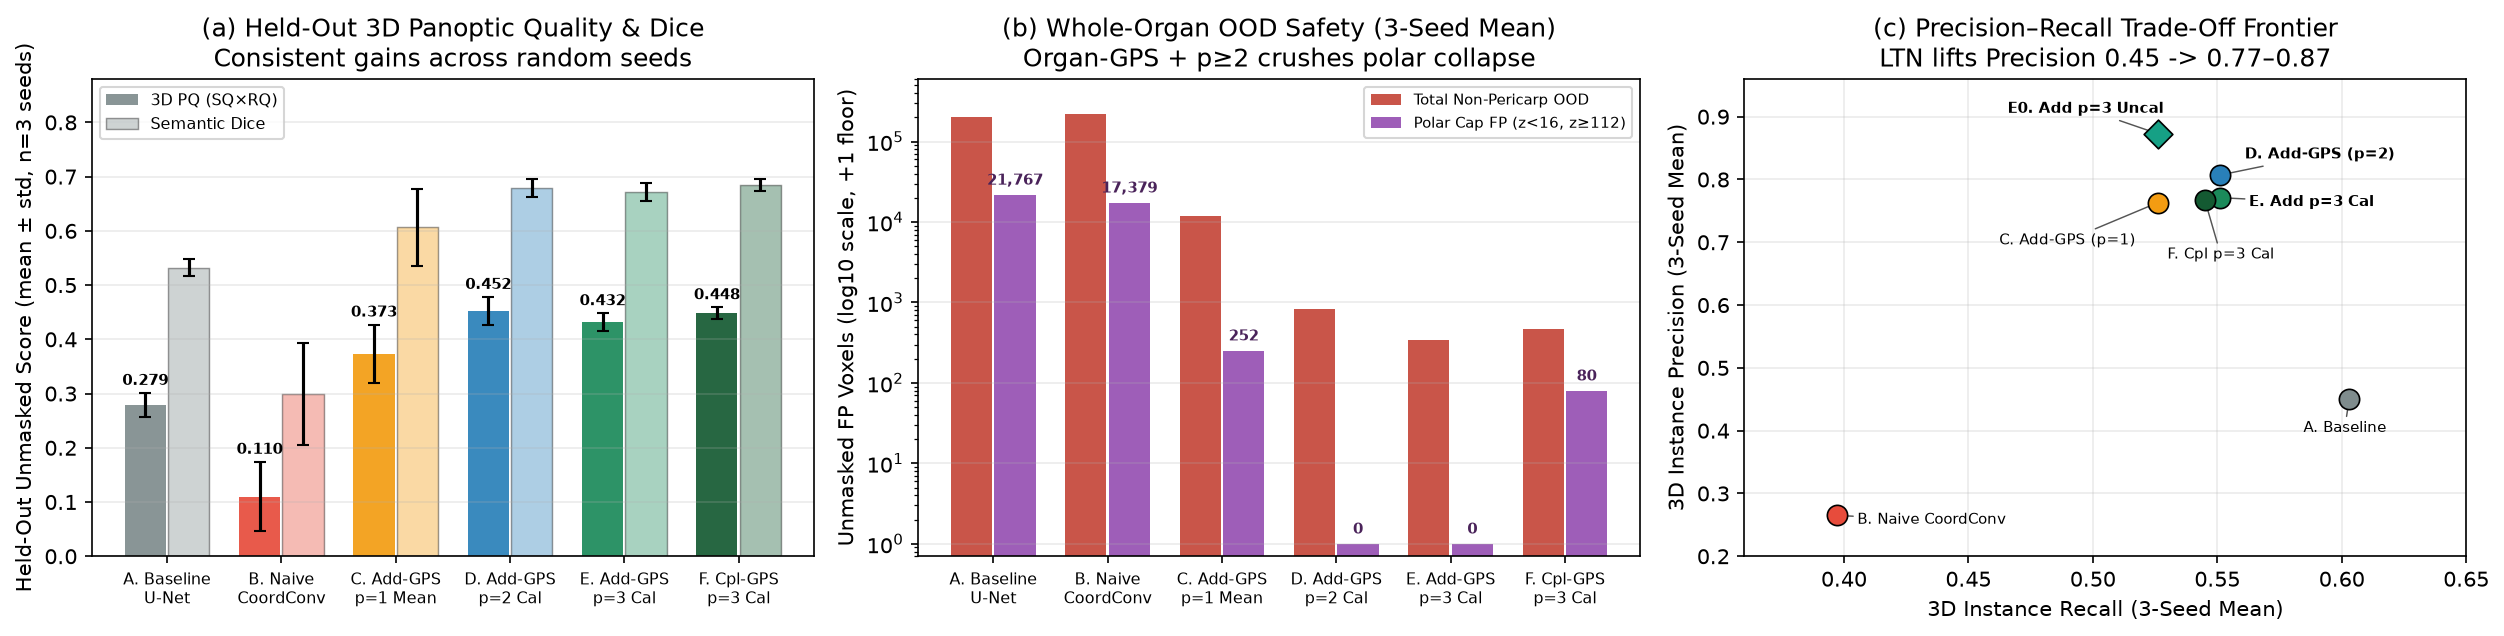
\includegraphics[width=\textwidth]{../figures/fig05_multiseed_ablation_benchmark.png}
    \vspace{-4pt}
    \caption*{\footnotesize\textit{Executed Figure~5 (\texttt{Out [3]}, saved as \texttt{fig05\_multiseed\_ablation\_benchmark.png}): 3-seed mean $\pm$ SD ablation benchmark comparing (a)~held-out 3D Panoptic Quality and Semantic Dice, (b)~unmasked 128-slice OOD and polar-cap false-positive voxels on a $\log_{10}$ scale ($21{,}767 \to 0$ polar FPs for Models~D/E), and (c)~the 3D instance Precision--Recall frontier.}}
\end{figure}
\begin{figure}[H]
    \centering
    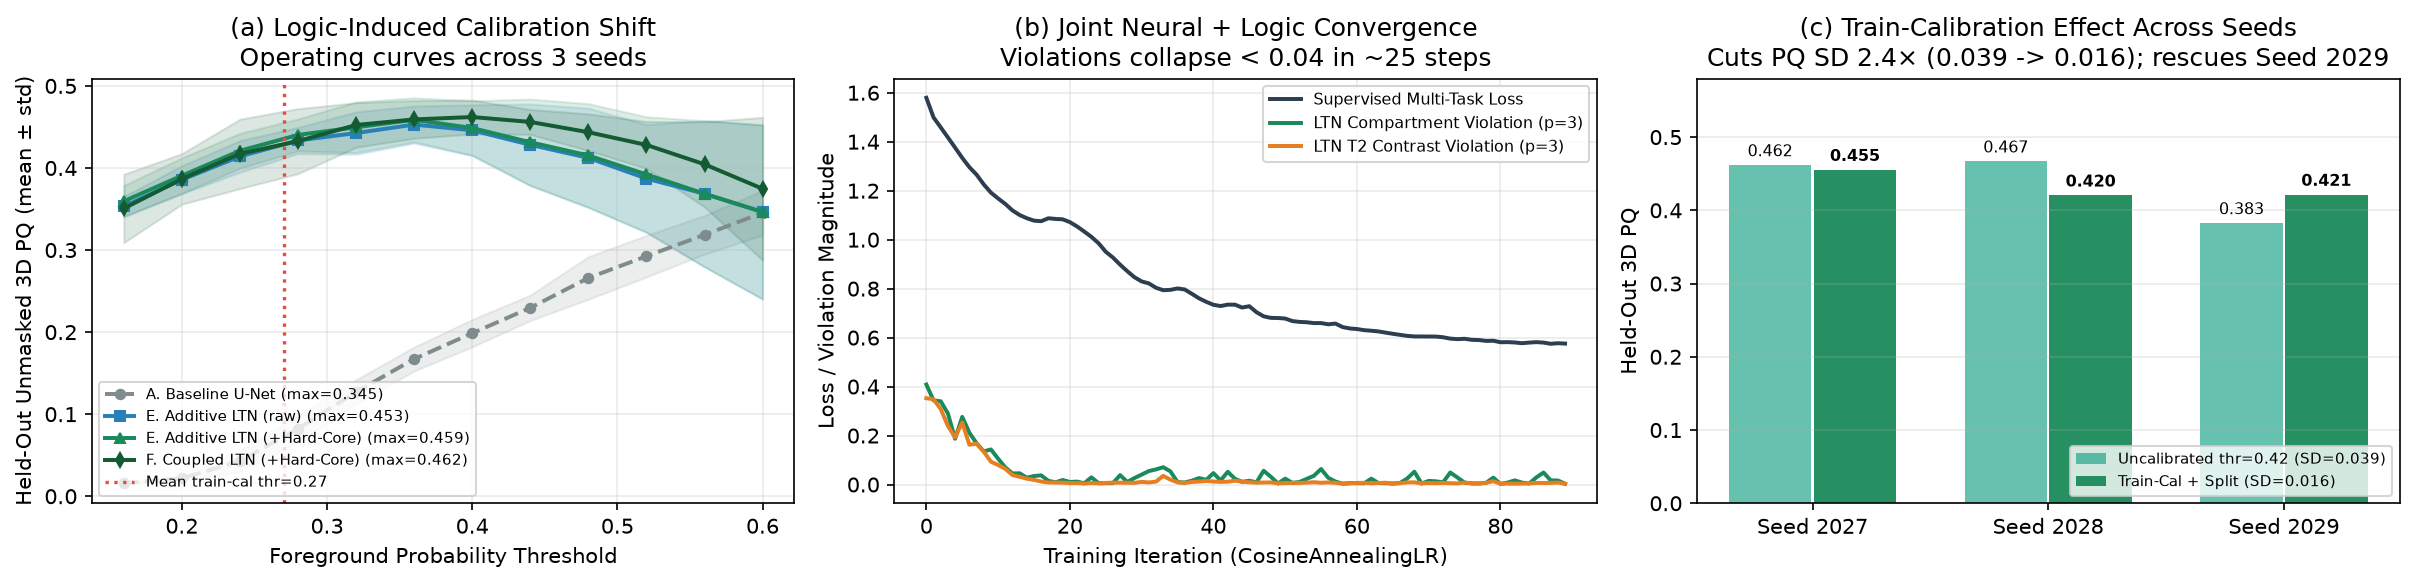
\includegraphics[width=\textwidth]{../figures/fig06_calibration_and_training_dynamics.png}
    \vspace{-4pt}
    \caption*{\footnotesize\textit{Executed Figure~6 (\texttt{Out [3]}, saved as \texttt{fig06\_calibration\_and\_training\_dynamics.png}): (a)~Logic-induced operating-curve shift $\text{PQ}(\tau_{\text{fg}})$ with $\pm 1$\,SD bands across seeds; (b)~joint supervised + $p = 3$ LTN convergence on Seed~2027; (c)~per-seed stabilization from uncalibrated $\tau = 0.42$ (\textbf{E0}) to train-calibrated + hard-core split (\textbf{E}), cutting $\text{PQ}$ SD $2.4\times$ ($0.039 \to 0.016$).}}
\end{figure}

\end{document}
